\documentclass{lni}

\IfFileExists{latin1.sty}{\usepackage{latin1}}{\usepackage{isolatin1}}

\usepackage{graphicx}

\author{Andreas Kn�pfle \& Tobias Schmid \\\\andreas.knoepfle@fu-berlin.de, tobias.schmid@fu-berlin.de}
\title{Eigennamenerkennung in mathematischen Texten}
\begin{document}
\maketitle

\begin{abstract}
abstract
\end{abstract}

\tableofcontents

\section{Einleitung}

\section{Grundlagen}
In mathematischen Texten k�nnen Standart-Tools zur Erkennung von Eigennamen, wie die von Personen, Organisationen oder Orten nicht verwendet werden, da die in die Mathematik eigene Eigennamen definiert. Beispielsweise gibt es Formeln, Gleichungen oder Theoreme wie z.B. Satz des Pythagoras oder das Bayestheorem, die eigene Namen tragen und oft in mathematischen Texten vorkommen. Die Erkennung dieser Eigennamen wurde in dieser Arbeit mit zwei unterschiedlichen Ans�tzen implementiert:
\begin{itemize}
	\item Regelbasierte Erkennung 
	\item Maschinelles Lernen
\end{itemize}
Bestehende Werkzeuge zur Eigennamenerkennung k�nnen zus�tzlich zur eigentlichen Erkennung der Eigennamen Label vergeben, die die Erkannten Eigennamen typisieren (z.B. erhalten erkannte Personennamen ein Person-Label). Da es aber in der Mathematik sehr viele verschiedene Konzepte gibt und sich die mathematischen Eigennamen oft vielen Konzepten zuordnen lassen, wurde in dieser Arbeit auf eine zus�tzliche Labelung der Eigenamen verzichtet. Die implementierten Ans�tze verwenden daher jeweils ein gemeinsames Label "MATH" f�r mathematische Entit�ten.
\subsection{Architektur}

\begin{figure}
  \begin{center}
  	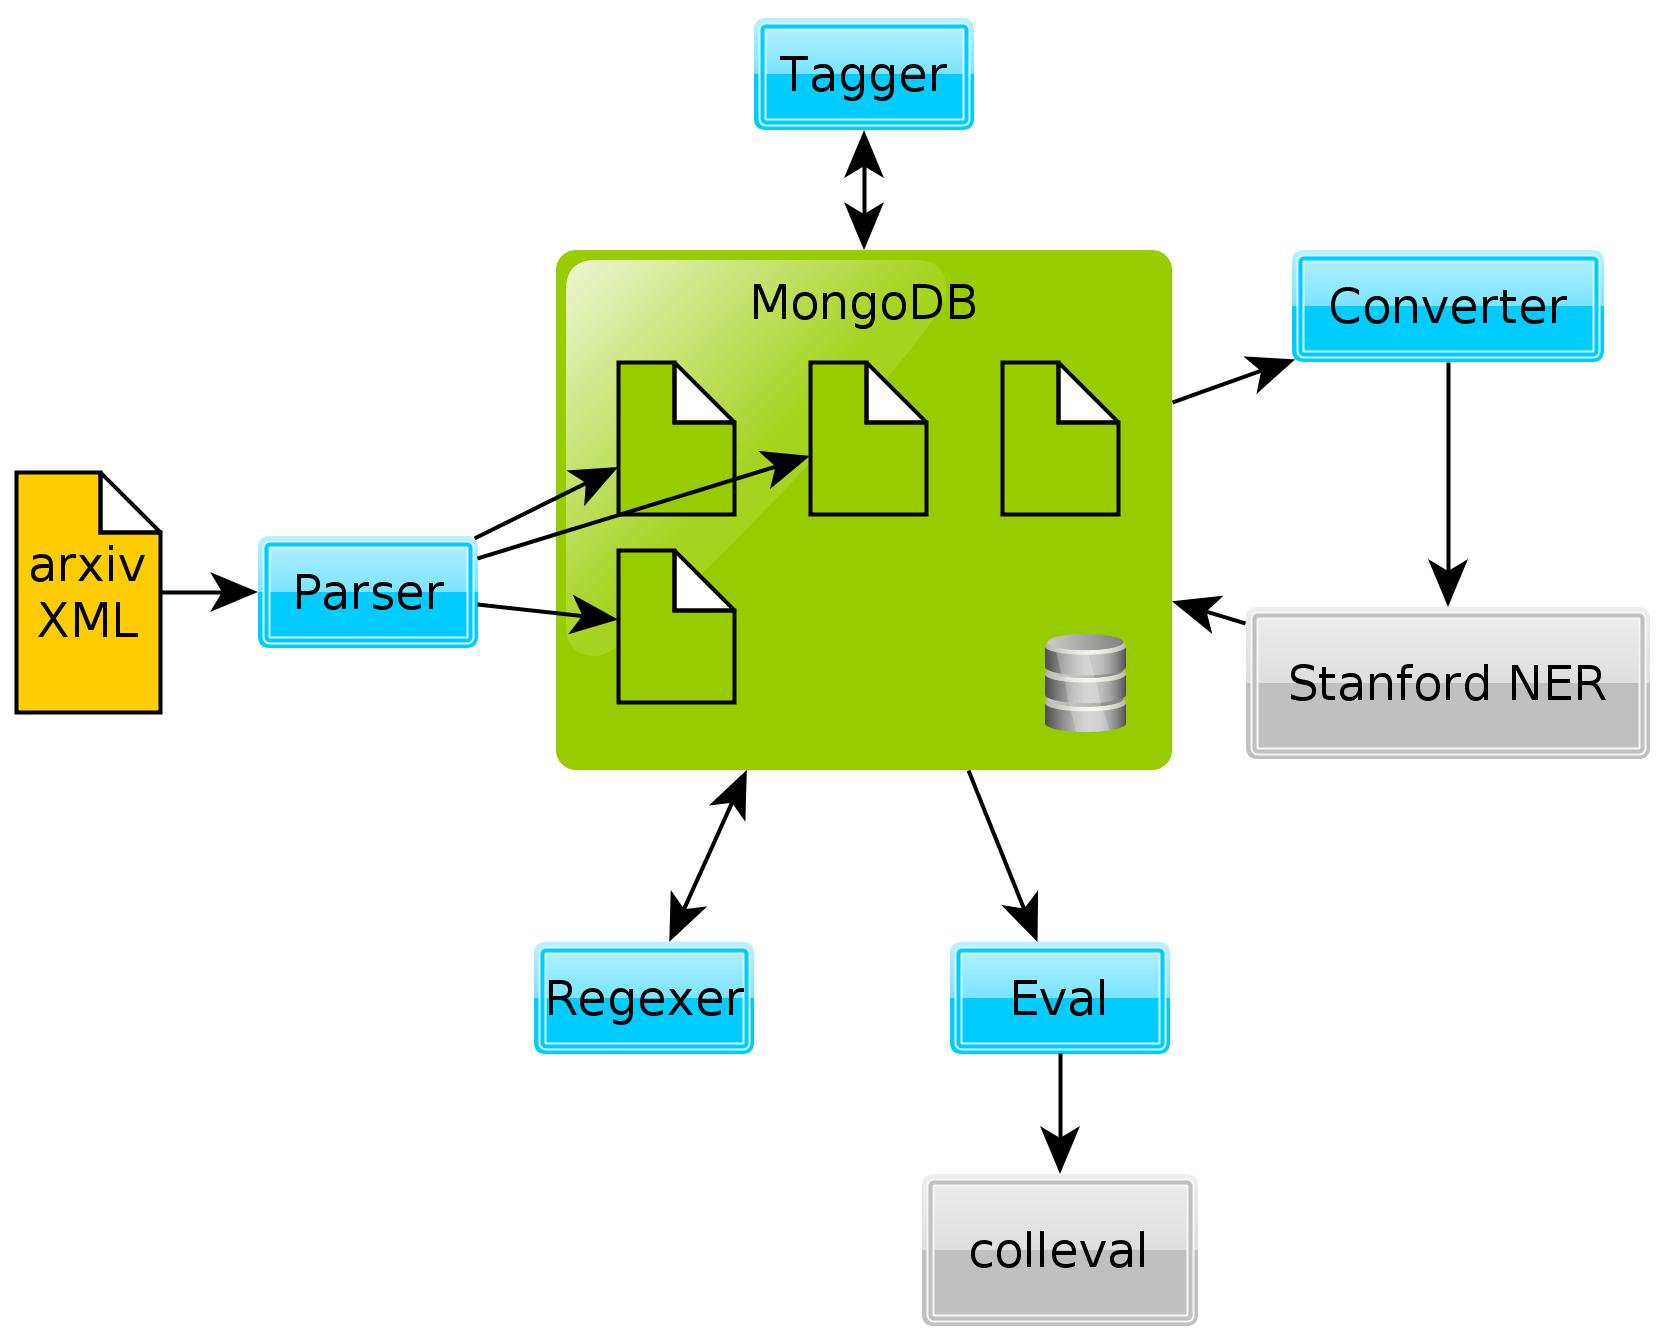
\includegraphics[width=0.7\textwidth]{image/arch.jpg}
  	\caption{Architektur der Evaluationsumgebung\label{arch}}
  \end{center}
\end{figure}


\subsection{Regelbasierte Erkennung}

\subsection{Erkennung mit maschinellem Lernen}

\subsection{Datensatz}


\subsection{Evaluationsmethoden}

\section{Analyse}

\subsection{Ergebnisse der Regelbasierte Erkennung}

\subsubsection*{Nicht erkannte Eigennamen}

\subsubsection*{Falsch erkannte Eigennamen}

\subsection{Ergebnisse der Erkennung mit maschinellem Lernen}

\subsubsection*{Nicht erkannte Eigennamen}

\subsubsection*{Falsch erkannte Eigennamen}

\section{Fazit}

\end{document}

